\subsection{Desconectarse de una partida}

\begin{figure}[ht]
\centering
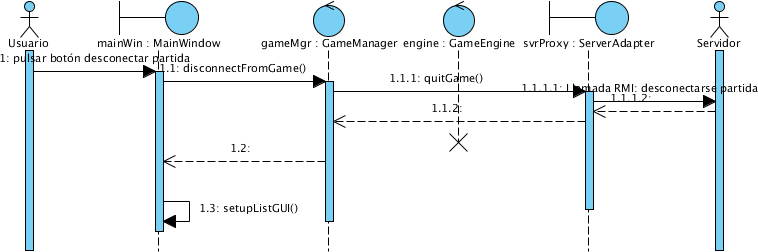
\includegraphics[scale=0.6]{img/ch03devel-exitgame.png}
\caption{Diagrama de secuencia de ``Desconectarse de una partida''}
\end{figure}

Un jugador puede en cualquier momento desconectarse de una partida. Esta
petición se realiza sobre el gestor de partidas, el cual notificará al servidor
la petición del usuario. A continuación eliminará el objeto de tipo
\texttt{GameEngine} creado cuando el usuario se conecto a la partida.

En un último paso, la ventana principal ejecuta la función
\texttt{setupListGUI} para volver a la vista con las listas de partidas.
